\documentclass[a4paper,10pt]{article}
\usepackage[utf8x]{inputenc}
\usepackage[T1]{fontenc}
\usepackage[french]{babel}

\usepackage{algorithmic}
\usepackage{algorithm}
\usepackage{graphicx}

\usepackage{common-formatting}
\usepackage{common-math}

%opening
\title{TP2 - Projets déterministes - MACS1}
\author{Alexandru Fikl}

\begin{document}

\maketitle

\section{Idée}
On cherche a résoudre $Ax = b$ via la construction d'une suite $x_k$ qui tende vers
$x$ lorsque $k \rightarrow \infty$. On étudie ici des méthodes itératives basés sur
la décomposition $(M, N)$ définie par $A = M − N$, avec $M$ facilemente inversible.
Ainsi, si $Ax = b$ alors on a $Mx = Nx + b$ et l'algorithme itératif sera:

\[
\left\{
\begin{array}{c}
x_0 \in \mathbb{K} \\
Mx_{k + 1} = Nx_k + b
\end{array}
\right.
\]

Soit:
\[
\left\{
\begin{array}{c}
x_0 \in \mathbb{K} \\
x_{k+1} = M^{-1}(Nx_{k} + b)
\end{array}
\right.
\]

\section{Jacobi}

Pour préciser cette méthode il suffit de préciser la décomposition $(M, N)$. Soit
$A = (a_{ij})$, on définit $M = D = a_{ij} \delta_{ij}$ . Donc
$N = M − A = D − A$. On suppose donc implicitement que ∀i $a_{ii} \neq 0$. (sinon $M$
n'est plus inversible)

\begin{prop}
Soit $A$ hermitienne définie positive (ou négative) et $2D − A$ définie positive
(ou négative), alors la méthode de Jacobi converge. A savoir: si $A$ est a diagonale
strictement dominante sur les lignes alors Jacobi converge aussi.
\end{prop}

\begin{enumerate}
    \item Ecrire la relation liant $x_{k+1}$ à $x_k$.
\[
Dx_{k + 1} = (D - A)x_k + b
\]

    \item Ecrire ce que vaut $x_{k+1,i}$ en fonction de $x_{k,i}$ (où $x_{k,i}$ représente la
composante $i$ à l'étape $k$).
\[
\forall i \in \llbracket 1, n \rrbracket, \;
x_{k + 1, i} = \frac{1}{a_{ii}}\left( b_i -
\sum_{\substack{
   j = 1 \\
   j \neq i
  }}^n a_{ij} x_{ki} \right)
\]

    \item Calculer le coût par itération de cette méthode.
\[
\underbrace{x_{k + 1, i} = \underbrace{\frac{1}{a_{ii}}\left( b_i -
\underbrace{\sum_{\substack{
   j = 1 \\
   j \neq i
  }}^n a_{ij} x_{ki}}_{2n - 3\; operations} \right)}_{(2n - 3) + 2\; operations}
}_{n(2n - 1)\; operations\; \forall i}
\]
Donc le coût est $T(n) = n (2n - 1) \in \mathcal{O}(n^2)$.

\hbox{}

On note le vecteur erreur a l’étape $k : e_k = x_k − x$. On note $r_k$ le résidu à l’étape $k$
définit de la manière suivante : $r_k = Ax_k − b$.

    \item Ecrire le pseudo-code de l'algorithme de Jacobi avec comme critére
    d'arrêt $\frac{\norm{r_k}{}}{\norm{b}{}} < \epsilon$. Pourquoi ce critére d'arrêt est
    légitime (formellement) ?

\begin{algorithm}
\caption{Algorithme de Jacobi}
\begin{algorithmic}
\STATE Données:
\STATE $A \in \mathcal{M}_{n, n}(\field{K})$
\STATE $b = \field{R}^n$
\STATE $x_0 = \field{R}^n$
\STATE Initialization:
\STATE $x_1 = 0 \in \field{R}^n$
\STATE $r_k = b$
\WHILE{$\frac{\norm{r_k}{}}{\norm{b}{}} < \epsilon$}
    \STATE $x_1(i) = \frac{1}{A(i, i)}\left( b_i - \sum_{\substack{
        j = 1 \\
        j \neq i
        }}^n A(i, j) x_0(i) \right).$
    \STATE $r_k = Ax_1 - b$.
    \STATE $x_0 = x_1$.
\ENDWHILE
\end{algorithmic}
\end{algorithm}

    Le critére d'arrêt est légitime parce que le résidu devient plus petit lorsque
    l'approximation $x_k$ tend à la solution $x$.

    \item Implémenter l'algorithme en matlab (sans oublier les commentaires).
    Changer le critére d'array et utiliser $\norm{e_k}{} = \norm{x_{k + 1} - x_k}{}
    < \epsilon$. Comparer. Ce critére est-il légitime ?

    \hbox{}

    (voir le fichier \emph{Jacobi.m} pour le code matlab).

    Ce critére est aussi légitime parce que l'erreur $e_k \to 0$ lorsque $x_k \to x$.

    \item Voir le fichier \emph{test\_iterative\_methods.m} et la Figure~\ref{fig:its}.

    \item Voir le fichier \emph{test\_iterative\_methods.m} et la Figure~\ref{fig:order}.
\end{enumerate}

\section{Gauss-Seidel}

Précisons la décomposition $(M, N)$. On pose $A = D - E - F$ où $D$ est la diagonale
de $A$, $-E$ est la partie triangulaire inférieure de $A$ et $-F$ sa partie supérieure.
On pose $M = D - E$ et $N = F$ donc on a $A = M - N$. On suppose aussi ici que
$\forall i,\, a_{ii} \neq 0$.

\begin{prop}
Soit A hermitienne définie positive (ou négative), alors la méthode de Gauss-Seidel
converge.
\end{prop}

\begin{enumerate}
    \item Ecrire la relation liant $x_{k+1}$ à $x_k$.
\[
(D - E)x_{k + 1} = F x_k + b
\]

    \item Ecrire ce que vaut $x_{k+1,i}$ en fonction de $x_{k,i}$ (où $x_{k,i}$ représente la
composante $i$ à l'étape $k$).
\[
\forall i \in \llbracket 1, n \rrbracket, \;
x_{k + 1, i} = \frac{1}{a_{ii}}
\left( b_i -
\sum_{j = 1}^{i - 1} a_{ij} x_{k + 1, j} -
\sum_{j = i + 1}^n a_{i, j} x_{k, j}
\right)
\]

    \item Calculer le coût par itération de cette méthode.
\[
\underbrace{x_{k + 1, i} = \underbrace{\frac{1}{a_{ii}}
\left( b_i -
\underbrace{\sum_{j = 1}^{i - 1} a_{i, j} x_{k + 1, j} -
\sum_{j = i + 1}^n a_{i, j} x_{k, j}}_{2n - 2\; operations}
\right)}_{2n\; operations}}_{n(2n)\; operations\; \forall i}
\]
Donc le coût est $T(n) = 2n^2 \in \mathcal{O}(n^2)$.

    \item Ecrire le pseudo-code de l'algorithme de Gauss-Seidel.

\begin{algorithm}
\caption{Algorithme de Gauss-Seidel}
\begin{algorithmic}
\STATE Données:
\STATE $A \in \mathcal{M}_{n, n}(\field{K})$
\STATE $b = \field{R}^n$
\STATE $x_0 = \field{R}^n$
\STATE Initialization:
\STATE $x_1 = 0 \in \field{R}^n$
\STATE $r_k = b$
\WHILE{$\frac{\norm{r_k}{}}{\norm{b}{}} < \epsilon$}
    \STATE $x_1(i) = \frac{1}{A(i, i)}
        \left( b_i -
            \sum_{j = 1}^{i - 1} A(i, j) x_1(j) -
            \sum_{j = i + 1}^n A(i, j) x_0(j)
        \right)$
    \STATE $r_k = Ax_1 - b$.
    \STATE $x_0 = x_1$.
\ENDWHILE
\end{algorithmic}
\end{algorithm}

    \item Voir le fichier \emph{GaussSeidel.m} pour le code matlab et la Figure~\ref{fig:its}.

    \item Voir le fichier \emph{test\_iterative\_methods.m}  et la Figure~\ref{fig:order}.

    \item La méthode de Gauss-Seidel converge plus rapidement que Jacobi
    parce que l'ordre de Gauss-Seidel est 2 tandis que l'ordre de Jacobi est 1.

\end{enumerate}

\section{S.O.R. (Succesive Over Relaxation)}

Précisons la décomposition $(M, N)$. On pose $A = D - E - F$ où $D$ est la diagonale
de $A$, $-E$ est la partie triangulaire inférieure de $A$ et $-F$ sa partie supérieure.
On pose $M = \frac{1}{\omega}D - E$ et $N = \frac{1 - \omega}{\omega}D + F$ donc on a
$A = M - N$. On suppose aussi ici que $\forall i,\, a_{ii} \neq 0$.

\begin{prop}
Soit $A$ une matrice symétrique définie positive. Si $\omega \in ]0, 2]$ alors la
méthode de relaxation S.O.R. converge pour toute donnée initiale.
\end{prop}

\begin{prop}
Soit A une matrice à diagonale strictement dominante ou irreductible à diagonale dominante.
Si $\omega \in ]0, 1]$ la méthode de relaxation S.O.R. converge pour toute donnée
initiale.
\end{prop}

\begin{prop}
Soit A une matrice tridiagonale et symétrique définie positive. La méthode relaxation
S.O.R. converge si et seulement si $0 < \omega < 2$. Le paramètre optimal est
\[
    \displaystyle \omega_opt = \frac{1}{1 + \sqrt{1 - \rho^2(J)}},
\]
où $J$ est la matrice de Jacobi.
\end{prop}

\begin{enumerate}
    \item Ecrire la relation liant $x_{k+1}$ à $x_k$.
\[
(\frac{1}{\omega}D - E)x_{k + 1} = (\frac{1 - \omega}{\omega}D + F) x_k + b
\]

    \item Ecrire ce que vaut $x_{k+1,i}$ en fonction de $x_{k,i}$ (où $x_{k,i}$ représente la
composante $i$ à l'étape $k$).
\[
\forall i \in \llbracket 1, n \rrbracket, \;
x_{k + 1, i} = \omega \hat{x}_{k+1, i} + (1 - \omega) x_{k, i}
\]
où $\hat{x}_{k+1, i}$ est donné par la méthode de Gauss-Seidel.

    \item Calculer le coût par itération de cette méthode: le coût est le même que
    pour Gauss-Seidel.

    \item Ecrire le pseudo-code de l'algorithme de S.O.R.

\begin{algorithm}
\caption{Algorithme de S.O.R.}
\begin{algorithmic}
\STATE Données:
\STATE $A \in \mathcal{M}_{n, n}(\field{K})$
\STATE $b = \field{R}^n$
\STATE $x_0 = \field{R}^n$
\STATE $\omega \in ]0, 2]$
\STATE Initialization:
\STATE $x_1 = 0 \in \field{R}^n$
\STATE $r_k = b$
\WHILE{$\frac{\norm{r_k}{}}{\norm{b}{}} < \epsilon$}
    \STATE calcul de $\hat{x}_1$ comme dans la méthode de Gauss-Seidel
    \STATE calcul de $x_1$ pour S.O.R. avec la formule
    $ x_1 = \omega \hat{x}_1 + (1 - \omega) x_0$
    \STATE $r_k = Ax_1 - b$.
    \STATE $x_0 = x_1$.
\ENDWHILE
\end{algorithmic}
\end{algorithm}

    \item Voir le fichier \emph{Relaxation.m} pour le code matlab et la Figure~\ref{fig:its}.

    \item Voir le fichier \emph{test\_iterative\_methods.m} et la Figure~\ref{fig:order}.

    \textbf{NOTE}: Dans la deuxième figure, l'ordre de chaque méthode est faux, sauf l'ordre
    de Jacobi. Je ne sais pas pourquoi parce qu'il est evident dans la prémière figure
    que Gauss-Seidel et S.O.R. converge plus vite que Jacobi.

\end{enumerate}

\begin{figure}[th!]
    \centering
    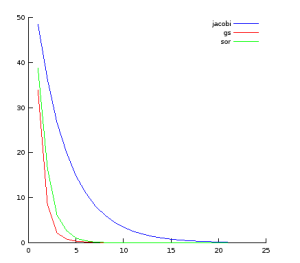
\includegraphics{./img/iterative-its.png}
    \caption{Iterations en fonction de l'erreur}
    \label{fig:its}
\end{figure}

\begin{figure}[th!]
    \centering
    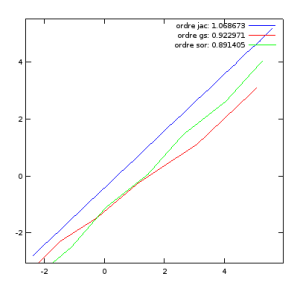
\includegraphics{./img/iterative-order.png}
    \caption{L'ordre de chaque méthode}
    \label{fig:order}
\end{figure}

\end{document}
